% ============================================================================
%  C1 Home-Based IoT Device Manager -- Deliverable #2 component design
%  Owner: Ekant Kapgate
% ============================================================================
\section{Component Overview}

\subsection{Purpose}
C1 Home-Based IoT Device Manager is the entry point of the clip-to-alert flow. It models each
tenant's houses and rooms, registers and configures camera feeds, ingests clips to object storage,
and manages each house's clip records. C1 owns steps 1 and 2 of the flow: it accepts an uploaded
clip for an enabled feed, writes the bytes to Amazon S3, and records the clip in the
\texttt{media\_events} collection with status \texttt{queued}. From there C3 takes over. C1 performs
no classification and raises no alerts.

A camera feed is a software-registered media source, not a physical device. Clips arrive as
uploaded audio or video files or as a phone-camera capture over HTTPS, so connectivity is a recorded
status derived from clip recency, not a measured radio metric.

\subsection{Objectives}
\begin{enumerate}
\item Model houses and rooms per tenant, and register, configure, assign, enable, disable and archive camera feeds.
\item Keep a version history of every feed configuration change, with restore.
\item Accept clip uploads only for enabled, room-assigned feeds; reject the rest with a precise error code.
\item Write each clip to the tenant/house prefix in S3 and record it as \texttt{queued} for C3, exactly once per clip.
\item Let staff and owners browse each house's clips (the Clip Library) and play them through short-lived signed links.
\item Record connectivity as a feed status derived from clip recency, never from hardware.
\end{enumerate}

\subsection{Function scope}
\begin{longtable}{L{6.4cm}L{8.4cm}}
\caption{C1 function scope}\label{tab:c1-scope}\\
\toprule
\textbf{In C1} & \textbf{Out of C1 (owner)} \\
\midrule
\endfirsthead
\caption[]{C1 function scope (continued)}\\
\toprule
\textbf{In C1} & \textbf{Out of C1 (owner)} \\
\midrule
\endhead
Houses, rooms, camera feeds, feed configuration versions & Classification and detections (C3) \\
Clip ingestion to S3 and \texttt{media\_events} (status \texttt{queued}) & Rule evaluation and alerts (C2) \\
Connectivity status, Clip Library and signed playback links & Authentication, users, RBAC token issue, dashboards (C4) \\
\bottomrule
\end{longtable}
\textbf{Assumptions.} C4 issues the JWT and C1 only verifies it against C4's published public key.
C3 updates the processing fields of \texttt{media\_events}; C1 never touches them after insert.

\subsection{Usage}
\begin{longtable}{L{3.0cm}L{4.0cm}L{7.8cm}}
\caption{C1 actors}\label{tab:c1-actors}\\
\toprule
\textbf{Actor} & \textbf{Interface} & \textbf{Typical use} \\
\midrule
\endfirsthead
\caption[]{C1 actors (continued)}\\
\toprule
\textbf{Actor} & \textbf{Interface} & \textbf{Typical use} \\
\midrule
\endhead
\texttt{iot\_staff} & \texttt{/iot/*} pages $\rightarrow$ C1 REST & Model houses and rooms; add, configure, enable, archive feeds; browse clips \\
\texttt{cloud\_staff} & C1 REST & Same as IoT staff, across tenants for support \\
\texttt{house\_owner} & My Feeds, Clip Library (read-only) & See own houses' feeds and play own clips \\
Upload client (device / phone) & \texttt{POST /ingest/clip} with an IoT service-account JWT & Post clips for an enabled feed \\
C3 inference worker & MongoDB \texttt{media\_events} & Claims \texttt{queued} clips; never calls C1 \\
\bottomrule
\end{longtable}

\subsection{Function partition}
Figure~\ref{fig:c1-partition} shows C1's five sub-functions; Table~\ref{tab:c1-fr} maps the requirements.

\figH{C1/c1-partition-overview}{0.58}{C1 function partition: five sub-functions under Home-Based IoT Device Manager}{fig:c1-partition}

\begin{longtable}{L{2.2cm}L{8.6cm}L{3.8cm}}
\caption{C1 functional requirements mapped to sub-functions}\label{tab:c1-fr}\\
\toprule
\textbf{Req} & \textbf{Requirement (abridged)} & \textbf{Sub-function} \\
\midrule
\endfirsthead
\caption[]{C1 functional requirements mapped to sub-functions (continued)}\\
\toprule
\textbf{Req} & \textbf{Requirement (abridged)} & \textbf{Sub-function} \\
\midrule
\endhead
FR-C1-01 & Create, update, delete houses and rooms inside the caller's tenant & House and room management \\
FR-C1-02 & Register a camera feed with name, media kind and capture configuration & Camera feed registration \\
FR-C1-03 & Update, delete and list feeds filtered by house, room, kind and status & Camera feed registration \\
FR-C1-04 & Version each configuration change; record connectivity status & Feed configuration and connectivity \\
FR-C1-05 & Assign a feed to one house and room; ingest, record and browse per-house clips & Clip ingestion; per-house data management \\
\bottomrule
\end{longtable}

\subsection{Component function specification}
\begin{longtable}{L{1.1cm}L{2.5cm}L{3.3cm}L{3.0cm}L{4.8cm}}
\caption{C1 function specification}\label{tab:c1-funcspec}\\
\toprule
\textbf{ID} & \textbf{Function} & \textbf{Input} & \textbf{Output} & \textbf{Pre- / post-conditions} \\
\midrule
\endfirsthead
\caption[]{C1 function specification (continued)}\\
\toprule
\textbf{ID} & \textbf{Function} & \textbf{Input} & \textbf{Output} & \textbf{Pre- / post-conditions} \\
\midrule
\endhead
F-01 & Manage houses & name, address, timezone, owner & House; 201/200/204 & Pre: staff in tenant. Delete only if the house has no enabled feeds (else 409); soft delete \\
F-02 & Manage rooms & house id, name, room type & Room & Pre: house in scope. Delete only if no feed is assigned to the room \\
F-03 & Register feed & name, kind, house, room?, config & CameraFeed (\texttt{provisioned}, disabled) & Post: config version 1 written \\
F-04 & Save / restore config & interval, sensitivity, label & FeedConfigVersion & Pre: $5 \le$ interval $\le 3600$ s. Post: \texttt{config\_version} = new version \\
F-05 & Enable / disable feed & feed id, \texttt{is\_enabled} & CameraFeed & Pre (enable): room assigned, else 409 \texttt{room\_required} \\
F-06 & Archive feed & feed id & 204 & Post: disabled, \texttt{archived\_at} set, clips kept \\
F-07 & Ingest clip & feed id, kind, captured\_at, file, client\_clip\_id? & MediaEvent \texttt{queued}; 201 & Pre: feed enabled + assigned; kind matches; $\le$ 50 MB. Post: one S3 object + one record \\
F-08 & Browse clips & house, feed, period, status & Page of clips & Post: only houses in caller scope \\
F-09 & Signed playback & media id & S3 URL valid 15 min & Pre: clip in caller scope \\
F-10 & Derive connectivity & (scheduled, 60 s) & connectivity, status & Post: Table~\ref{tab:c1-dt-conn} applied to every enabled feed \\
\bottomrule
\end{longtable}

% ============================================================================
\section{Component Application Interface Design and Analysis}

\subsection{API conventions}
Paths are relative to \texttt{https://<host>/api/v1}; JSON over HTTPS with \texttt{Authorization: Bearer <JWT>}
issued by C4 (claims \texttt{sub}, \texttt{role}, \texttt{tenant\_id}, \texttt{house\_ids}). Success bodies use
\texttt{\{"data": ..., "meta": \{"page", "page\_size", "total"\}\}}; errors use
\texttt{\{"error": \{"code", "message", "details"\}\}}. Lists are paged (\texttt{page}, \texttt{page\_size} $\le$ 100).
IDs are UUID strings, including \texttt{media\_id}. Times are ISO-8601 UTC. The OpenAPI contract is frozen at Deliverable~\#2.

\subsection{API catalogue}
\begin{longtable}{L{1.3cm}L{4.9cm}L{2.8cm}L{1.2cm}L{4.4cm}}
\caption{C1 API catalogue}\label{tab:c1-catalogue}\\
\toprule
\textbf{Method} & \textbf{Path} & \textbf{Access} & \textbf{OK} & \textbf{Purpose} \\
\midrule
\endfirsthead
\caption[]{C1 API catalogue (continued)}\\
\toprule
\textbf{Method} & \textbf{Path} & \textbf{Access} & \textbf{OK} & \textbf{Purpose} \\
\midrule
\endhead
GET, POST & \texttt{/houses} & staff & 200, 201 & List / create houses \\
GET, PATCH, DELETE & \texttt{/houses/\{id\}} & staff (owner: GET) & 200, 204 & Read / edit / soft-delete a house \\
GET, POST & \texttt{/houses/\{id\}/rooms} & staff (owner: GET) & 200, 201 & List / create rooms \\
PATCH, DELETE & \texttt{/rooms/\{id\}} & staff & 200, 204 & Rename / delete a room \\
GET, POST & \texttt{/feeds} & staff (owner: GET) & 200, 201 & List with filters / register a feed \\
GET, PATCH, DELETE & \texttt{/feeds/\{id\}} & staff (owner: GET) & 200, 204 & Read / rename or reassign room / archive \\
PATCH & \texttt{/feeds/\{id\}/status} & staff & 200 & Enable or disable \\
PUT & \texttt{/feeds/\{id\}/config} & staff & 200 & Save a new config version \\
GET & \texttt{/feeds/\{id\}/config-versions} & staff & 200 & Version history \\
POST & \texttt{/feeds/\{id\}/\allowbreak config-versions/\allowbreak\{v\}/restore} & staff & 200 & Restore version \texttt{v} as a new version \\
POST & \texttt{/ingest/clip} & iot\_staff, cloud\_staff, upload service account & 201 & Upload a clip \\
GET & \texttt{/clips} & staff, owner & 200 & Clip Library list \\
GET & \texttt{/clips/\{media\_id\}} & staff, owner & 200 & One clip record and status \\
GET & \texttt{/clips/\{media\_id\}/\allowbreak playback-url} & staff, owner, C2/C3 service & 200 & Signed S3 GET URL (15 min) \\
\bottomrule
\end{longtable}

\subsection{Web service API: POST /feeds}
Registers a camera feed. The feed starts \texttt{provisioned} and disabled, and config version 1 is written.
\begin{longtable}{L{2.8cm}L{1.4cm}L{1.6cm}L{1.1cm}L{7.0cm}}
\caption{POST /feeds body}\\
\toprule
\textbf{Parameter} & \textbf{In} & \textbf{Type} & \textbf{Req.} & \textbf{Description} \\
\midrule
\endfirsthead
\caption[]{POST /feeds body (continued)}\\
\toprule
\textbf{Parameter} & \textbf{In} & \textbf{Type} & \textbf{Req.} & \textbf{Description} \\
\midrule
\endhead
\texttt{name} & body & string & yes & 1--80 chars, unique within the house \\
\texttt{media\_kind} & body & string & yes & \texttt{audio} or \texttt{video} \\
\texttt{house\_id} & body & uuid & yes & Owning house, in the caller's tenant \\
\texttt{room\_id} & body & uuid & no & Room of that house; required before Enable \\
\texttt{config.capture\_interval\_s} & body & int & yes & 5--3600 \\
\texttt{config.sensitivity} & body & string & yes & \texttt{low}, \texttt{medium}, \texttt{high} (capture sensitivity, not alert sensitivity) \\
\texttt{config.network\_label} & body & string & no & Free text, recorded only \\
\bottomrule
\end{longtable}

\subsection{Web service API: PUT /feeds/\{id\}/config and restore}
\texttt{PUT /feeds/\{id\}/config} takes the three \texttt{config} fields above and appends version $n+1$.
\texttt{POST /feeds/\{id\}/config-versions/\{v\}/restore} copies version \texttt{v} into a new version, so history
is never rewritten. Both return \texttt{\{config\_version, config\}}; 404 for an unknown version, 422 for a bad interval.

\subsection{Web service API: POST /ingest/clip}
Uploads a clip for an enabled feed and records it as \texttt{queued}. The server generates \texttt{media\_id}.
An optional \texttt{client\_clip\_id} makes retries safe: a repeat for the same feed returns the first record.
\begin{longtable}{L{2.8cm}L{1.6cm}L{1.6cm}L{1.1cm}L{6.8cm}}
\caption{POST /ingest/clip parameters}\\
\toprule
\textbf{Parameter} & \textbf{In} & \textbf{Type} & \textbf{Req.} & \textbf{Description} \\
\midrule
\endfirsthead
\caption[]{POST /ingest/clip parameters (continued)}\\
\toprule
\textbf{Parameter} & \textbf{In} & \textbf{Type} & \textbf{Req.} & \textbf{Description} \\
\midrule
\endhead
\texttt{feed\_id} & form & uuid & yes & Target feed; must be enabled and room-assigned \\
\texttt{media\_kind} & form & string & yes & Must match the feed's kind \\
\texttt{captured\_at} & form & date-time & yes & Capture time (UTC); not more than 5 min in the future \\
\texttt{client\_clip\_id} & form & string & no & Client idempotency key, unique per feed \\
\texttt{file} & multipart & binary & yes & \texttt{audio/wav}, \texttt{audio/mpeg} or \texttt{video/mp4}; $\le$ 50 MB \\
\bottomrule
\end{longtable}
\begin{Shaded}
\begin{Code}
POST /api/v1/ingest/clip   (multipart: feed_id, media_kind=audio, captured_at, client_clip_id, file)
201 Created { "data": { "media_id": "9b1e2f40-6c3d-4e1a-9f0b-2c8d1a7e5b07", "status": "queued",
                        "s3_key": "tenants/0b6e/houses/a3d9/feeds/e2f4/2026/10/24/9b1e2f40.wav",
                        "duplicate": false } }
\end{Code}
\end{Shaded}
\noindent Errors: \texttt{404 not\_found} (no such feed in scope), \texttt{409 feed\_not\_enabled} (disabled or no room),
\texttt{413 payload\_too\_large}, \texttt{422 media\_kind\_mismatch} / \texttt{validation\_error}, \texttt{503 storage\_unavailable}.

\subsection{Web service API: GET /clips and playback URL}
\texttt{GET /clips} filters by \texttt{house\_id}, \texttt{feed\_id}, \texttt{from}, \texttt{to} and \texttt{status}
(\texttt{queued}, \texttt{processing}, \texttt{analyzed}, \texttt{failed}) and returns media id, feed, room, capture time,
size and status. \texttt{GET /clips/\{media\_id\}/playback-url} returns \texttt{\{url, expires\_at\}} where the URL is an
S3 pre-signed GET valid for 15 minutes. C2's Alert Detail and signed alert view use this endpoint with a service JWT.

\subsection{Error model}
\begin{longtable}{L{1.3cm}L{4.2cm}L{9.2cm}}
\caption{C1 error codes}\\
\toprule
\textbf{HTTP} & \textbf{code} & \textbf{When} \\
\midrule
\endfirsthead
\caption[]{C1 error codes (continued)}\\
\toprule
\textbf{HTTP} & \textbf{code} & \textbf{When} \\
\midrule
\endhead
401 / 403 & \texttt{unauthorized} / \texttt{forbidden} & Bad or expired token; role or house outside scope \\
404 & \texttt{not\_found} & Unknown house, room, feed, version or clip in scope \\
409 & \texttt{feed\_not\_enabled}, \texttt{room\_required}, \texttt{house\_not\_empty}, \texttt{room\_in\_use} & State rule broken (Tables~\ref{tab:c1-dt-ingest}, \ref{tab:c1-dt-delete}) \\
413 / 422 & \texttt{payload\_too\_large} / \texttt{validation\_error}, \texttt{media\_kind\_mismatch} & File or field invalid \\
503 & \texttt{storage\_unavailable} & S3 or MongoDB unavailable; nothing is left half-written \\
\bottomrule
\end{longtable}

\subsection{Connectivity APIs}
\begin{longtable}{L{3.2cm}L{2.6cm}L{2.4cm}L{6.4cm}}
\caption{C1 connectivity interfaces}\label{tab:c1-conn}\\
\toprule
\textbf{Interface} & \textbf{Protocol / port} & \textbf{Auth} & \textbf{Data exchanged} \\
\midrule
\endfirsthead
\caption[]{C1 connectivity interfaces (continued)}\\
\toprule
\textbf{Interface} & \textbf{Protocol / port} & \textbf{Auth} & \textbf{Data exchanged} \\
\midrule
\endhead
Clients $\rightarrow$ C1 REST & HTTPS 443 via ALB & User / service JWT & All endpoints above (inbound) \\
C1 $\rightarrow$ Amazon S3 & HTTPS 443 (AWS SDK) & IAM instance role & PUT clip at \texttt{tenants/\{t\}/\allowbreak houses/\{h\}/\allowbreak feeds/\{f\}/\allowbreak yyyy/mm/dd/\allowbreak\{media\_id\}.\{ext\}} with SSE; presigned GET \\
C1 $\rightarrow$ MongoDB \texttt{media\_events} & TCP 27017 & Per-service DB user & Insert clip record \texttt{queued}; this collection is the queue C3 reads \\
C1 $\rightarrow$ PostgreSQL (own) & TCP 5432 & Secrets Manager & \texttt{houses}, \texttt{rooms}, \texttt{camera\_feeds}, \texttt{feed\_config\_versions} \\
C1 $\leftarrow$ C4 JWKS & HTTPS 443 & Public & Public key to verify JWTs (cached 10 min) \\
C3 / C4 $\rightarrow$ C1 stores & TCP, read-only users & Secrets Manager & C3 record browsing and C4 statistics read C1 data; never write \\
\bottomrule
\end{longtable}

\subsection{API design analysis}
\begin{longtable}{L{2.8cm}L{12.0cm}}
\caption{C1 API design decisions}\\
\toprule
\textbf{Concern} & \textbf{Decision and rationale} \\
\midrule
\endfirsthead
\caption[]{C1 API design decisions (continued)}\\
\toprule
\textbf{Concern} & \textbf{Decision and rationale} \\
\midrule
\endhead
Exactly-once ingest & Server-generated \texttt{media\_id}; optional \texttt{client\_clip\_id} unique per feed; S3 write first, then the record, and the object is deleted if the insert fails. A clip is never queued without bytes. \\
Security & Every query filters on the token's \texttt{tenant\_id} and \texttt{house\_ids}; S3 objects are private and encrypted; playback only through 15-minute signed URLs. \\
Loose coupling & The handoff to C3 is the \texttt{queued} record, not a call, so C1 keeps accepting clips while C3 is busy or down. \\
History & Config changes and restores append versions; feeds and houses are archived or soft-deleted, so clips and alerts stay traceable. \\
\bottomrule
\end{longtable}

% ============================================================================
\section{Component Function Design, Data and DB Design, and Behavior Analysis}

\subsection{Class design}
Figure~\ref{fig:c1-class} shows controllers, domain services, the scheduled \texttt{ConnectivityMonitor}, the
\texttt{S3MediaGateway}, the repositories and the domain models. Table~\ref{tab:c1-classspec} specifies them.

\begin{landscape}
\centering
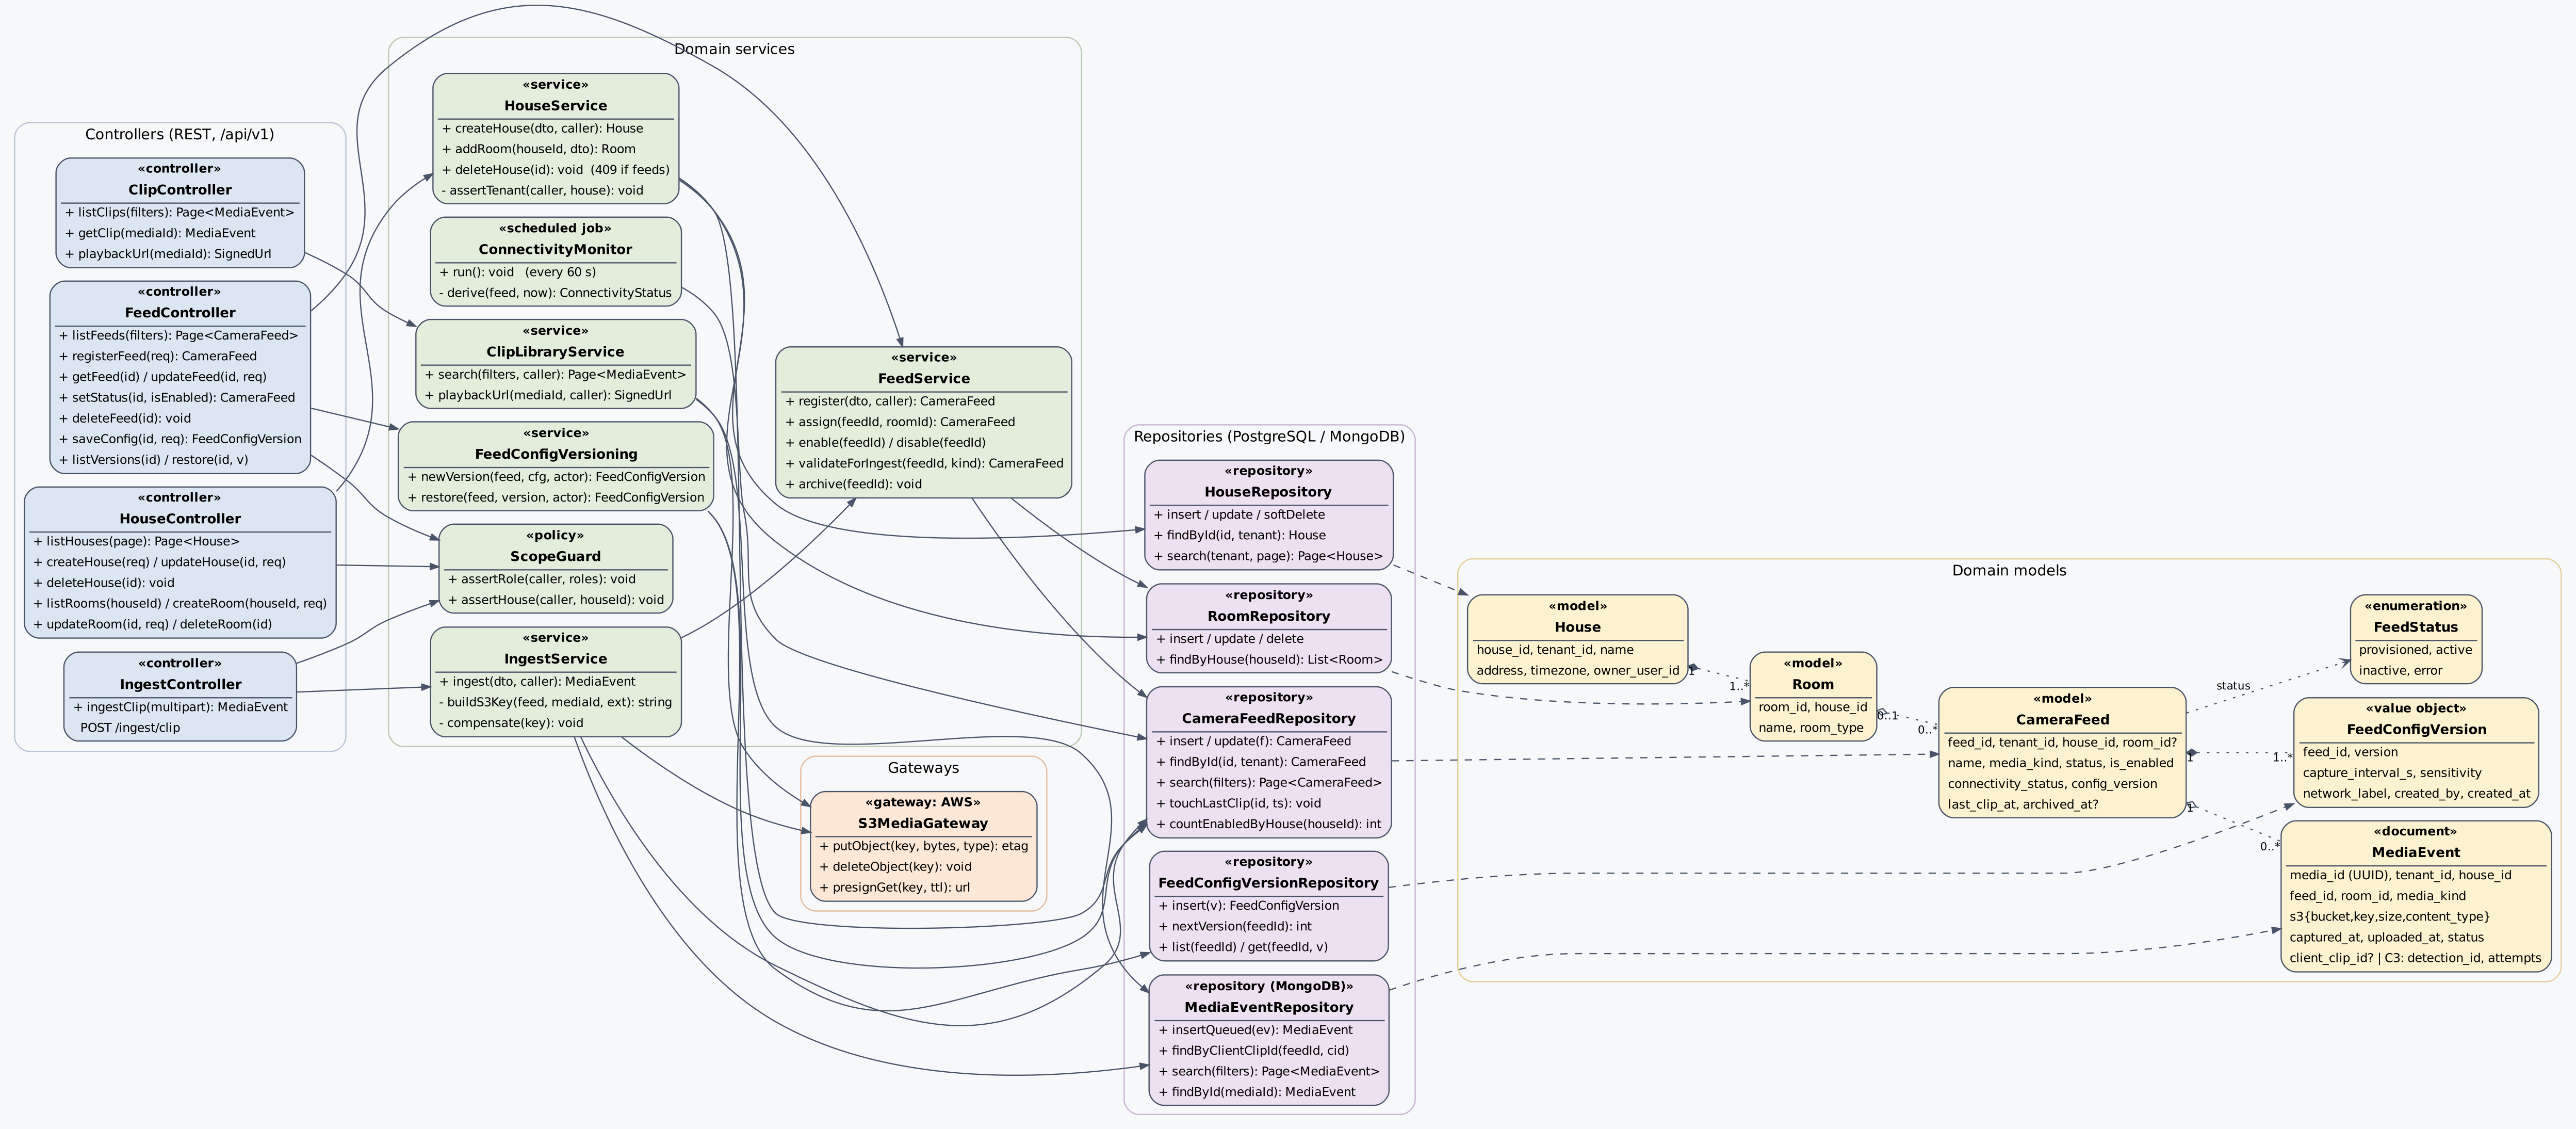
\includegraphics[width=\linewidth,height=0.86\textheight,keepaspectratio]{figures/C1/c1-class}
\captionof{figure}{C1 internal class diagram (dashed arrow = manages model; diamonds = aggregation / composition)}\label{fig:c1-class}
\end{landscape}

\begin{longtable}{L{3.6cm}L{1.9cm}L{5.8cm}L{3.5cm}}
\caption{C1 class specification}\label{tab:c1-classspec}\\
\toprule
\textbf{Class} & \textbf{Type} & \textbf{Responsibility} & \textbf{Uses} \\
\midrule
\endfirsthead
\caption[]{C1 class specification (continued)}\\
\toprule
\textbf{Class} & \textbf{Type} & \textbf{Responsibility} & \textbf{Uses} \\
\midrule
\endhead
\texttt{House-, Feed-, Ingest-, ClipController} & controller & Map REST calls to services; map errors to HTTP codes & \texttt{ScopeGuard}, services \\
\texttt{ScopeGuard} & policy & Role and tenant/house checks from JWT claims & JWT claims \\
\texttt{HouseService} & service & Houses and rooms; delete guards & House/Room/Feed repositories \\
\texttt{FeedService} & service & Register, assign, enable/disable, archive; \texttt{validateForIngest} & \texttt{CameraFeedRepository} \\
\texttt{FeedConfigVersioning} & service & Append and restore config versions & \texttt{FeedConfigVersion\allowbreak Repository} \\
\texttt{IngestService} & service & Validate, idempotency, S3 write, queued record, compensation & \texttt{FeedService}, \texttt{S3MediaGateway}, \texttt{MediaEventRepository} \\
\texttt{ClipLibrary\allowbreak Service} & service & Scoped clip search; signed playback URL & \texttt{MediaEventRepository}, \texttt{S3MediaGateway} \\
\texttt{ConnectivityMonitor} & job (60 s) & Derive \texttt{connectivity\_status} and \texttt{active}/\texttt{inactive} & \texttt{CameraFeedRepository} \\
\texttt{S3MediaGateway} & gateway & put, delete, presign & Amazon S3 \\
\bottomrule
\end{longtable}

\subsection{Data and database design}
C1 owns four PostgreSQL tables and the \texttt{media\_events} MongoDB collection (Figure~\ref{fig:c1-er}).

\figH{C1/c1-er}{1.0}{C1 entity-relationship diagram (white = C1-owned, grey = other components)}{fig:c1-er}

\begin{longtable}{L{4.6cm}L{3.0cm}L{7.0cm}}
\caption{C1 data dictionary (key columns)}\label{tab:c1-dd}\\
\toprule
\textbf{Table.column} & \textbf{Type} & \textbf{Constraint / description} \\
\midrule
\endfirsthead
\caption[]{C1 data dictionary (key columns) (continued)}\\
\toprule
\textbf{Table.column} & \textbf{Type} & \textbf{Constraint / description} \\
\midrule
\endhead
\texttt{houses.house\_id}, \texttt{tenant\_id} & UUID & PK; tenant from C4. \texttt{timezone} is an IANA zone used for quiet hours \\
\texttt{rooms.room\_type} & VARCHAR CHECK & \texttt{bedroom}, \texttt{kitchen}, \texttt{living}, \texttt{bathroom}, \texttt{entry}, \texttt{other} \\
\texttt{camera\_feeds.media\_kind} & VARCHAR CHECK & \texttt{audio}, \texttt{video} \\
\texttt{camera\_feeds.status} & VARCHAR CHECK & \texttt{provisioned}, \texttt{active}, \texttt{inactive}, \texttt{error} \\
\texttt{camera\_feeds.is\_enabled} & BOOLEAN & Separate from status; default false \\
\texttt{camera\_feeds.connectivity\_status} & VARCHAR CHECK & \texttt{online}, \texttt{offline}, \texttt{unknown} \\
\texttt{camera\_feeds.config}, \texttt{config\_version} & JSONB, INT & Copy of the current version \\
\texttt{camera\_feeds.consecutive\_failures} & SMALLINT & Reset on success; 3 sets \texttt{error} \\
\texttt{feed\_config\_versions} & PK (feed\_id, version) & Append-only; \texttt{capture\_interval\_s} CHECK 5--3600 \\
\texttt{media\_events.\_id} & UUID string & \texttt{media\_id}; also \texttt{tenant\_id}, \texttt{house\_id}, \texttt{room\_id}, \texttt{feed\_id}, \texttt{media\_kind}, \texttt{s3}, \texttt{captured\_at}, \texttt{uploaded\_at} \\
\texttt{media\_events.status} & string & \texttt{queued} at insert; C3 moves it to \texttt{processing}, \texttt{analyzed}, \texttt{failed} \\
\bottomrule
\end{longtable}
\textbf{Indexes.} \texttt{camera\_feeds(tenant\_id, house\_id, status)}; \texttt{UNIQUE camera\_feeds(house\_id, name)};
\texttt{media\_events \{status:1, uploaded\_at:1\}} (C3 queue); \texttt{\{house\_id:1, captured\_at:-1\}} (Clip Library);
\texttt{UNIQUE \{feed\_id:1, client\_clip\_id:1\}} (sparse). S3 objects move to infrequent access after 30 days and expire after 1 year.

\subsection{Program function descriptions}
\begin{longtable}{L{4.0cm}L{3.8cm}L{6.8cm}}
\caption{C1 key internal functions}\label{tab:c1-fn}\\
\toprule
\textbf{Function} & \textbf{Inputs $\rightarrow$ outputs} & \textbf{Logic} \\
\midrule
\endfirsthead
\caption[]{C1 key internal functions (continued)}\\
\toprule
\textbf{Function} & \textbf{Inputs $\rightarrow$ outputs} & \textbf{Logic} \\
\midrule
\endhead
\texttt{IngestService.\allowbreak ingest} & upload $\rightarrow$ MediaEvent & Validate feed and file, idempotency, S3 put, insert \texttt{queued}, compensate on failure \\
\texttt{FeedService.\allowbreak enable} & feed $\rightarrow$ feed & Requires \texttt{room\_id}; sets \texttt{is\_enabled} \\
\texttt{FeedConfigVersioning.\allowbreak newVersion} & feed, cfg $\rightarrow$ version & Insert $n+1$ and copy into \texttt{camera\_feeds} in one transaction \\
\texttt{ConnectivityMonitor.\allowbreak derive} & feed, now $\rightarrow$ status & Table~\ref{tab:c1-dt-conn} \\
\texttt{HouseService.\allowbreak deleteHouse} & house $\rightarrow$ void & 409 if any enabled feed; else soft delete \\
\texttt{ClipLibraryService.\allowbreak playbackUrl} & media id $\rightarrow$ URL & Scope check, presign 15 min \\
\bottomrule
\end{longtable}

\figH{C1/c1-ingest-flow}{0.62}{Clip ingestion flowchart: auth, scope, enable and room check, file check, idempotency, S3 write, record, compensation}{fig:c1-ingest}

\begin{Shaded}
\begin{Code}
function ingest(req, caller):
    feed = feeds.findById(req.feed_id, caller.tenant_id)      ; if not feed: raise 404 not_found
    scope.assertHouse(caller, feed.house_id)
    if not feed.is_enabled or feed.room_id is None:          raise 409 feed_not_enabled
    if req.media_kind != feed.media_kind:                     raise 422 media_kind_mismatch
    if req.file.size > 50 MB or req.file.type not in ALLOWED: raise 413 / 422
    if req.client_clip_id and (ev := mediaEvents.findByClientClipId(feed.id, req.client_clip_id)):
        return ok(ev, duplicate=True)
    media_id = uuid4()
    key = f"tenants/{feed.tenant_id}/houses/{feed.house_id}/feeds/{feed.id}/{ymd(req.captured_at)}/{media_id}.{ext}"
    s3.putObject(key, req.file, sse=True)                      # 503 storage_unavailable on error
    try:
        ev = mediaEvents.insertQueued(_id=media_id, tenant_id=feed.tenant_id, house_id=feed.house_id,
                 room_id=feed.room_id, feed_id=feed.id, media_kind=req.media_kind, s3={bucket, key, size, type},
                 captured_at=req.captured_at, uploaded_at=now(), client_clip_id=req.client_clip_id, status="queued")
    except DbError:
        s3.deleteObject(key); raise 503 storage_unavailable     # compensate: no orphan object
    feeds.touchLastClip(feed.id, req.captured_at)              # provisioned/inactive -> active, failures = 0
    return created(ev)

function derive(feed, now):                                    # ConnectivityMonitor, every 60 s
    if feed.last_clip_at is None:                       return ("unknown", feed.status)
    if now - feed.last_clip_at <= feed.config.capture_interval_s: return ("online", "active")
    return ("offline", "inactive" if feed.status != "error" else "error")
\end{Code}
\end{Shaded}

\subsection{Behavior: feed state machine}
Figure~\ref{fig:c1-state} is the feed state machine; Table~\ref{tab:c1-dt-state} lists the transitions. A new feed is
\texttt{provisioned}. Once assigned and enabled, its first accepted clip makes it \texttt{active}; no clip within the
capture interval makes it \texttt{inactive}; three consecutive ingest failures (S3 error or unreadable file) set
\texttt{error}. \texttt{is\_enabled} is separate from status: a disabled feed keeps its status but rejects uploads.

\figH{C1/c1-feed-state}{0.52}{Camera feed state machine: provisioned, active, inactive, error}{fig:c1-state}

\subsection{Behavior: sequence diagrams}
Figure~\ref{fig:c1-seq} is Upload a clip (UC-02): C1 validates the feed, writes the bytes, records the clip as
\texttt{queued} and returns; the C3 worker claims it later. Figure~\ref{fig:c1-seq-feed} is Register, configure and
enable a feed, including the \texttt{409 room\_required} branch.

\figH{C1/c1-seq-upload}{0.95}{Sequence (a): upload a clip (UC-02); C1 boundary ends at status queued}{fig:c1-seq}
\figH{C1/c1-seq-feed}{0.95}{Sequence (b): IoT staff register, configure and enable a feed}{fig:c1-seq-feed}

% ============================================================================
\section{Component Business Logic}

\subsection{Clip ingestion decision table}
\begin{longtable}{L{1.7cm}L{2.2cm}L{1.9cm}L{2.4cm}L{2.0cm}L{4.2cm}}
\caption{Clip ingestion}\label{tab:c1-dt-ingest}\\
\toprule
\textbf{Feed in scope} & \textbf{Enabled + room} & \textbf{Kind matches} & \textbf{Type/size OK} & \textbf{Dup. client id} & \textbf{Action} \\
\midrule
\endfirsthead
\caption[]{Clip ingestion (continued)}\\
\toprule
\textbf{Feed in scope} & \textbf{Enabled + room} & \textbf{Kind matches} & \textbf{Type/size OK} & \textbf{Dup. client id} & \textbf{Action} \\
\midrule
\endhead
no & -- & -- & -- & -- & \texttt{404 not\_found} \\
yes & no & -- & -- & -- & \texttt{409 feed\_not\_enabled} \\
yes & yes & no & -- & -- & \texttt{422 media\_kind\_mismatch} \\
yes & yes & yes & no & -- & \texttt{413} / \texttt{422} \\
yes & yes & yes & yes & yes & 200, return existing record \\
yes & yes & yes & yes & no & 201: S3 write, insert \texttt{queued} \\
\bottomrule
\end{longtable}

\subsection{Connectivity derivation decision table}
\begin{longtable}{L{6.4cm}L{3.0cm}L{5.0cm}}
\caption{Connectivity derivation (every 60 s)}\label{tab:c1-dt-conn}\\
\toprule
\textbf{Condition} & \textbf{connectivity\_status} & \textbf{status effect} \\
\midrule
\endfirsthead
\caption[]{Connectivity derivation (every 60 s) (continued)}\\
\toprule
\textbf{Condition} & \textbf{connectivity\_status} & \textbf{status effect} \\
\midrule
\endhead
No clip ever received & \texttt{unknown} & stays \texttt{provisioned} \\
Last clip within one capture interval & \texttt{online} & \texttt{active} \\
Last clip older than one interval & \texttt{offline} & \texttt{inactive} (unless \texttt{error}) \\
\bottomrule
\end{longtable}

\subsection{Feed status transition table}
\begin{longtable}{L{2.6cm}L{5.4cm}L{2.4cm}L{4.2cm}}
\caption{Feed status transitions}\label{tab:c1-dt-state}\\
\toprule
\textbf{From} & \textbf{Event / guard} & \textbf{To} & \textbf{Action} \\
\midrule
\endfirsthead
\caption[]{Feed status transitions (continued)}\\
\toprule
\textbf{From} & \textbf{Event / guard} & \textbf{To} & \textbf{Action} \\
\midrule
\endhead
(new) & \texttt{POST /feeds} & \texttt{provisioned} & Version 1, disabled \\
\texttt{provisioned} & First clip accepted (enabled + room) & \texttt{active} & \texttt{last\_clip\_at} set \\
\texttt{active} & No clip within interval & \texttt{inactive} & connectivity \texttt{offline} \\
\texttt{inactive} & Clip accepted & \texttt{active} & connectivity \texttt{online} \\
any & 3 consecutive ingest failures & \texttt{error} & Shown in Camera Feed Manager \\
\texttt{error} & Staff re-enable after fix & \texttt{provisioned} & Failures reset \\
\bottomrule
\end{longtable}

\subsection{Delete and enable guards}
\begin{longtable}{L{4.4cm}L{5.0cm}L{5.2cm}}
\caption{Delete and enable guards}\label{tab:c1-dt-delete}\\
\toprule
\textbf{Request} & \textbf{Condition} & \textbf{Result} \\
\midrule
\endfirsthead
\caption[]{Delete and enable guards (continued)}\\
\toprule
\textbf{Request} & \textbf{Condition} & \textbf{Result} \\
\midrule
\endhead
Enable feed & \texttt{room\_id} is null & \texttt{409 room\_required} \\
Delete house & any enabled feed in house & \texttt{409 house\_not\_empty} \\
Delete room & any feed assigned to room & \texttt{409 room\_in\_use} \\
Archive feed & always allowed & disabled; clips and versions kept \\
\bottomrule
\end{longtable}

\subsection{Access decision table}
\begin{longtable}{L{5.2cm}L{3.0cm}L{3.0cm}L{3.4cm}}
\caption{C1 access by role}\\
\toprule
\textbf{Operation} & \textbf{iot\_staff} & \textbf{cloud\_staff} & \textbf{house\_owner} \\
\midrule
\endfirsthead
\caption[]{C1 access by role (continued)}\\
\toprule
\textbf{Operation} & \textbf{iot\_staff} & \textbf{cloud\_staff} & \textbf{house\_owner} \\
\midrule
\endhead
Create / edit houses, rooms, feeds, configs & own tenant & any tenant & no (403) \\
Upload clips & own tenant & any tenant & no \\
List feeds, clips; playback & own tenant & any tenant & own houses only \\
\bottomrule
\end{longtable}

% ============================================================================
\section{Component Graphic User Interface Design}

\subsection{GUI style}
\begin{longtable}{L{3.0cm}L{11.8cm}}
\caption{C1 GUI style}\\
\toprule
\textbf{Element} & \textbf{Rule} \\
\midrule
\endfirsthead
\caption[]{C1 GUI style (continued)}\\
\toprule
\textbf{Element} & \textbf{Rule} \\
\midrule
\endhead
Workspace & IoT staff pages under \texttt{/iot/*} in the shared React SPA shell from C4; owners see read-only My Feeds and Clip Library under \texttt{/home/*}. \\
Status encoding & Feed status as icon + word (filled dot \texttt{active}, half dot \texttt{inactive}, open dot \texttt{provisioned}, cross \texttt{error}); connectivity as dot + label + age, never colour alone. \\
Forms & Add/Edit feed opens a side panel with inline validation from the 422 \texttt{details}; Enable is disabled with a hint while no room is set. \\
Destructive actions & Disable and Archive are outlined red and need a confirm dialog. \\
Accessibility & WCAG 2.1 AA contrast, keyboard operation, table headers announced. \\
\bottomrule
\end{longtable}

\subsection{Storyboard}
Figure~\ref{fig:c1-story}: in path~A, IoT staff open Camera Feed Manager (1), add a feed (2), assign and enable it (3),
and see it turn \texttt{active} after its first clip (4). In path~B, a device uploads a clip (5), C1 validates and
queues it (6), and staff or owners browse (7) and play it (8).

\figH{C1/c1-storyboard}{1.0}{C1 storyboard: feed setup and clip upload / Clip Library}{fig:c1-story}

\subsection{Function partition tree}
\figH{C1/c1-gui-tree}{0.55}{C1 GUI function partition: pages and their function buttons}{fig:c1-gui-tree}

\subsection{UI markup diagram and wireframe}
Figure~\ref{fig:c1-wireframe} is Camera Feed Manager with the Add feed panel; Table~\ref{tab:c1-markup} explains the callouts.

\figH{C1/c1-wireframe-feedmgr}{0.9}{UI markup of Camera Feed Manager with the Add feed panel}{fig:c1-wireframe}

\begin{longtable}{L{0.6cm}L{3.2cm}L{2.6cm}L{3.8cm}L{4.4cm}}
\caption{Camera Feed Manager markup legend}\label{tab:c1-markup}\\
\toprule
\textbf{\#} & \textbf{Element} & \textbf{Template} & \textbf{Data source} & \textbf{Behaviour} \\
\midrule
\endfirsthead
\caption[]{Camera Feed Manager markup legend (continued)}\\
\toprule
\textbf{\#} & \textbf{Element} & \textbf{Template} & \textbf{Data source} & \textbf{Behaviour} \\
\midrule
\endhead
1 & Top navigation & AppShell (C4) & JWT role & IoT links only for staff \\
2 & Filter bar + Add feed & FilterBar & \texttt{GET /houses}, rooms & Filters drive \texttt{GET /feeds} query \\
3 & Feeds table & DataTable, StatusChip & \texttt{GET /feeds} & Paged; row opens Feed Detail \\
4 & Add feed panel & FormPanel & \texttt{POST /feeds} & Inline 422 errors; room hint \\
5 & Feed action bar & ActionBar & feed status & Edit config, Versions, Clip Library, Disable, Archive (confirm) \\
\bottomrule
\end{longtable}

\subsection{GUI templates}
\begin{longtable}{L{3.0cm}L{4.2cm}L{7.6cm}}
\caption{GUI templates used by C1}\\
\toprule
\textbf{Template} & \textbf{Used on} & \textbf{Props / behaviour} \\
\midrule
\endfirsthead
\caption[]{GUI templates used by C1 (continued)}\\
\toprule
\textbf{Template} & \textbf{Used on} & \textbf{Props / behaviour} \\
\midrule
\endhead
AppShell (C4) & all pages & Role-aware navigation, breadcrumb, toasts \\
DataTable & Feeds, Clip Library, Versions & Server-side paging and sort \\
FilterBar & Feeds, Clip Library & House, room, kind, status, date range \\
StatusChip & Feeds, clips & Icon + word for feed and clip status \\
FormPanel & Add / Edit feed, config & Field validation from 422 \texttt{details} \\
ClipPlayer & Clip Library & Plays the signed playback URL \\
\bottomrule
\end{longtable}
